	On considère la fonction $f$ définie sur l'intervalle $]-1 ;+\infty[$ par :
	\[f(x)=a+\dfrac{b \ln (x+1)}{x+1}.\]
	où $a$ et $b$ sont des réels, et ln désigne la fonction logarithme népérien.

	On admet que la fonction $f$ est deux fois dérivable sur $]-1 ; +\infty [$.

	On note $f'$ sa fonction dérivée et $f''$ sa fonction dérivée seconde.

	\subsection*{Partie A}
	L'objectif de cette partie est de déterminer les valeurs de $a$ et $b$ de sorte que la courbe représentative de la fonction $f$ sur $]-1 ;+\infty[$ %changement : dans l'énoncé, c'était écrit $[0 ; +\infty[$, mais la fonction est définie plus largement et la courbe présente des abscisses strictement négatives.
	corresponde à celle tracée dans le repère orthonormé ci-dessous :

	\begin{center}
		%%Figure en tikz
		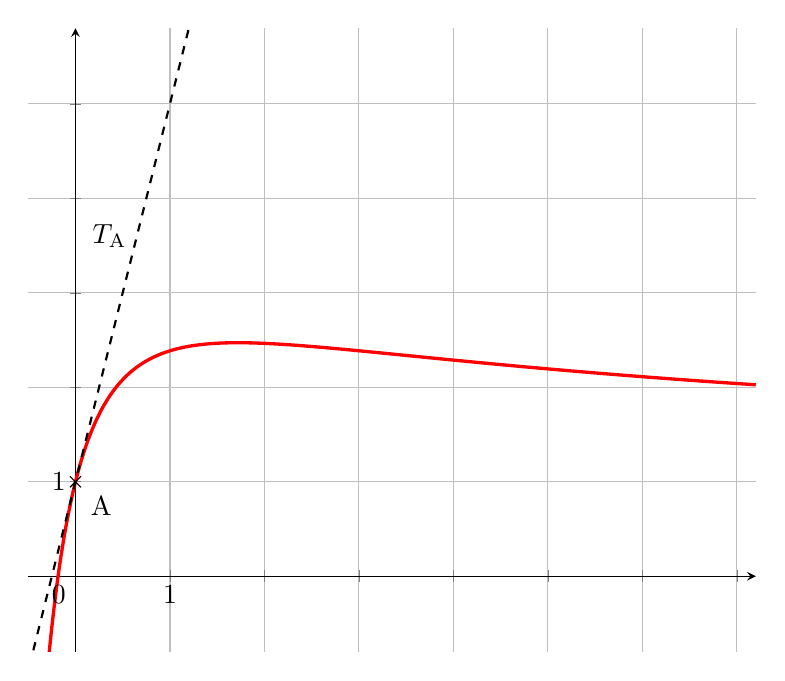
\begin{tikzpicture}%compiler avec pgfplots
			\begin{axis}[/pgf/number format/.cd, use comma,
				x={12mm}, y={12mm},
				xmin = -0.5, xmax = 7.2,
				ymin = -0.8, ymax = 5.8,
				xtick distance=1, ytick distance=1,
				xticklabels={},yticklabels={},
				minor tick num = 0,
				grid=major, axis lines =center]
				\addplot [line width=1.2pt,color=red,smooth,samples=100,domain= -0.5:7.2 ]{1+(4*ln(x+1))/(x+1)};
				\node[below left] at (axis cs: 0,0) {0};
				\node[below] at (axis cs: 1,0) {1};
				\node[left] at (axis cs: 0,1) {1};
				\draw[shift={(axis cs: 0,1)}] (2pt,2pt)--(-2pt,-2pt) (-2pt,2pt)--(2pt,-2pt) node[below right]{A};
				\draw[dashed,line width=0.8pt] (axis cs: -1,-3)--(axis cs: 2,9) node[pos=0.55,left] {$T_{\mathrm{A}}$} ;
%				\node at(axis cs: ) {$ \mathcal{C}_f $};
			\end{axis}
		\end{tikzpicture}
%		%%Figure en pstricks
%		\psset{xunit=1cm,yunit=1cm,arrowsize=2pt 3,comma}
%		\def\xmin {-0.8}   \def\xmax {7.2}
%		\def\ymin {-0.8}   \def\ymax {5.8}
%		\begin{pspicture*}(\xmin,\ymin)(\xmax,\ymax)\psgrid[yunit=1cm,subgriddiv=1,  gridlabels=0, gridcolor=lightgray]
%			\psaxes[labelFontSize=\footnotesize,labels=none, ticksize=-2pt 2pt,]{->}(0,0)(\xmin,\ymin)(\xmax,\ymax)
%			%\psset{linecolor=red,fillstyle=solid,fillcolor=pink!50}
%			\psplot[linecolor=blue,linewidth=1.2pt,plotpoints=5000]{\xmin}{\xmax}{1 4 x 1 add ln mul x 1 add div add}
%			\psplot[linecolor=red,linestyle=dashed,linewidth=1.2pt,plotpoints=5000]{\xmin}{\xmax}{1 4 x mul add}
%			\rput(0.3,3.5){\red $T_{\text A}$}
%			\uput[-10](0,1){A} \uput*[dl](0,0){O}
%			\uput[l](0,1){1} \uput[d](1,0){1}
%		\end{pspicture*}
	\end{center}


	On précise que la droite $T_{\mathrm{A}}$ est la tangente à la courbe représentative de la fonction $f$ au point A$(0 ; 1)$.

	\begin{enumerate}
		\item Justifier que $a=1$.

		\item En utilisant le graphique :
		\begin{enumerate}
			\item Donner la valeur de $f'(0)$.

			Justifier.
			\item Donner le signe de $f''(1)$.

			Justifier.
		\end{enumerate}

		\item \begin{enumerate}
			\item Montrer que pour tout réel $x$ appartenant à $]-1 ;+\infty[$, on a :
			\[f'(x)=\dfrac{b(1-\ln (x+1))}{(x+1)^{2}}\]

			\item En déduire la valeur de $b$.
		\end{enumerate}
	\end{enumerate}


	\subsection*{Partie B}
	On admet dans la suite de l'exercice que la fonction $f$ est définie sur $]-1 ;+\infty[$ par :
	\[f(x)=1+\dfrac{4 \ln (x+1)}{x+1}\]

	\begin{enumerate}
		\item Justifier que la droite d'équation \quad $y=1$ \quad est asymptote à la courbe représentative de la fonction~$f$.

		\item Résoudre l'inéquation \quad $1-\ln (x+1)>0$ \quad sur $]-1 ;+\infty[$.

		\item On admet que \quad $\lim\limits_{x \to -1} f(x)=-\infty$.

		Dresser le tableau de variation complet de la fonction $f$ en indiquant la valeur exacte de son extremum.

		Justifier.

		\item Montrer que l'équation \quad $f(x)=1,5$ \quad admet une unique solution dans l'intervalle $[2 ; +\infty[$.

		En donner une valeur arrondie à $10^{-1}$.

		\item \begin{enumerate}
			\item Montrer que :
			\[\int_{0}^{2} \dfrac{\ln (x+1)}{x+1} \d x=\dfrac{1}{2}\big(\ln 3\big)^{2}.\]

			\item En déduire l'aire, en unité d'aire, du domaine délimité par l'axe des abscisses, la courbe représentative de la fonction $f$, l'axe des ordonnées et la droite d'équation \quad $x=2$.
		\end{enumerate}
	\end{enumerate}
